\section{PV generation}

The phenomenon in which the transformation of solar energy to electrical energy is based is known as the \textit{Photovoltaic effect}. This  was first discovered by a French physicist named Edmond Becquerel in 1839. It is based on the emission, from the sunlight or light, of massless photons which collide on two superimposed layers of semiconductor material, causing some of the electrons to flow. This process allows the generation of electrics power. 

Solar PV cells are made of a negative charged layer (n-layer) and a positive charged layer (p-layer) of a semiconductor material, usually crystalline silicon, joined establishing a p-n junction. If photons collide with the n-layer and they have enough energy to excite the electrons, an electric field will be formed in the p-n junction due to the attraction of electrons and holes. This electric field will work as a diode permitting the separation of the positive and negative charge carriers. This way electric current will flow across the p-n junction allowing the generation of electric energy. %[https://www.ab.gov.tr/files/ardb/evt/1_avrupa_birligi/1_9_politikalar/1_9_6_enerji_politikasi/2009_report-solar-energy.pdf]
The greater the intensity of the light (irradiance) that is absorbed by the PV panel, the higher the amount of electric power generated. On the other hand, the efficiency of the panel will decrease with the temperature. Usually, PV panels are tested under standard test conditions (STC) which is at 25$\dec$C and 1000 $W/ m^2$. %[ http://www.sabz-energy.com/solar%20electricity%20handbook%202017.pdf]
Some of the most important characteristics associated with a PV panel’s datasheet are the following: maximum power ($P_{max}$), open-circuit voltage ($V_{oc}$), short-circuit current ($I_{sc}$), MPP voltage ($V_{mpp}$), MPP current ($I_{mpp}$) and efficiency ($\eta$).  %[ http://www.sabz-energy.com/solar%20electricity%20handbook%202017.pdf]
These features are important to define the I-V curves of the PV panel in order to develop the MPPT controller unit. Figure \ref{fig:PVsystemblocks} shows a block diagram with the main parts of a PV system.

\begin{figure}[htbp]
	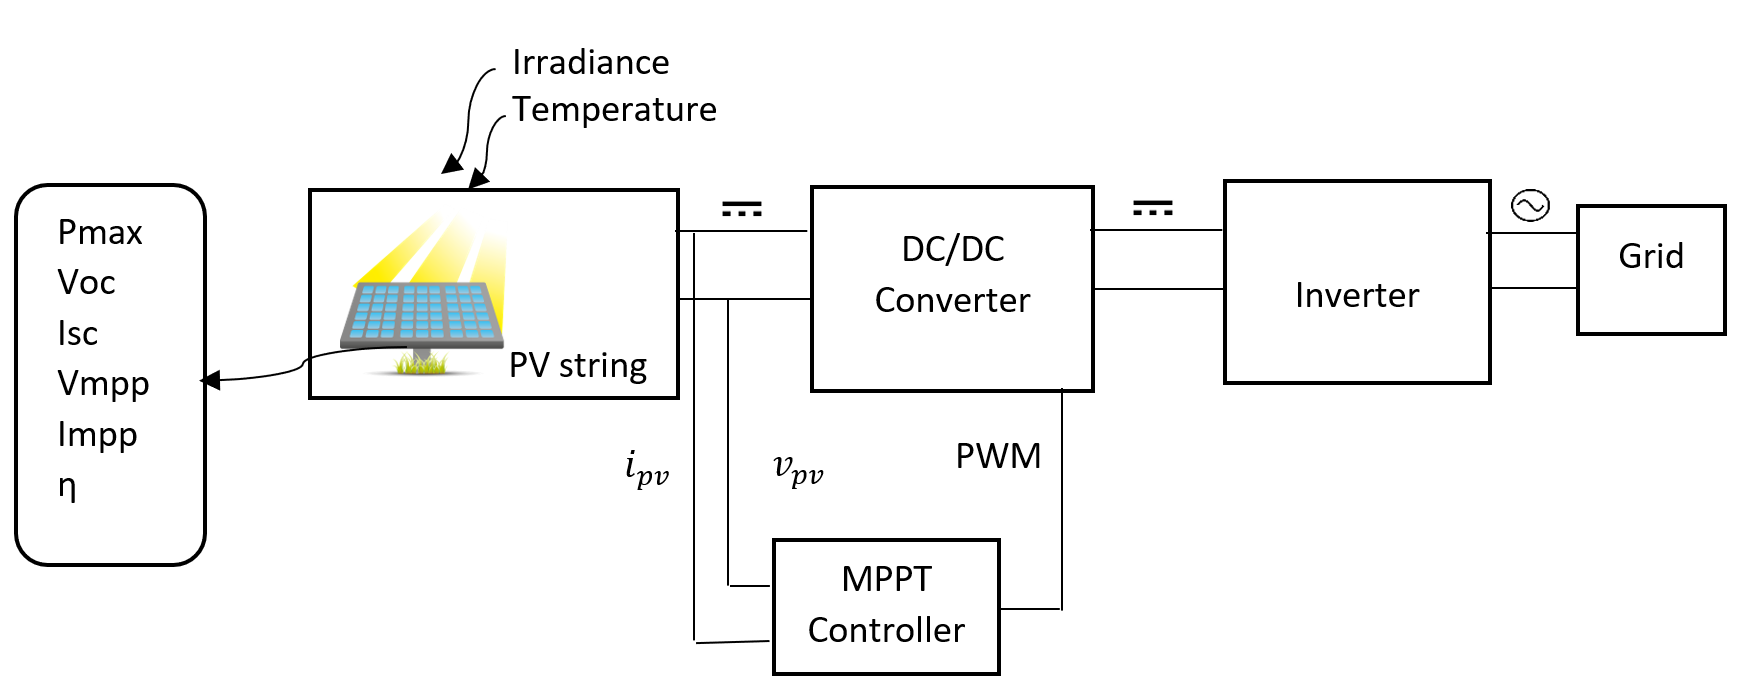
\includegraphics[width=\linewidth]{../Pictures/PV_system_blocks}
	\caption{Basic diagram of a PV grid-tie with battery backup system.}
	\label{fig:PVsystemblocks}
\end{figure}

PV systems can be classified in three main types: off-grid, grid-tie and grid-tie with battery backup (hybrid) systems. Off-grid systems are not connected to the grid which means that the power generated by the PV modules is stored in a battery bank for later use. In grid-tie systems the DC current is converted, using an inverter, into an AC current compatible with the grid. Nowadays, grid-tie systems are the most common, however, their main disadvantage is that they do not have battery backup. Which means that if there is a power outage the PV system will also be cut.  The solution to this problem is the grid-hybrid system which is a combination of a grid-tie system with a bank of batteries. This way it is possible to store energy and there is a battery backup in case of power outage. %[http://www.sabz-energy.com/solar%20electricity%20handbook%202017.pdf]
